\documentclass[twocolumn,11pt,a4paper]{article}
\usepackage[utf8]{inputenc}
\usepackage[T1]{fontenc}
\usepackage[numbers]{natbib}
\usepackage{color}
\usepackage{listings}
\usepackage{ amssymb }
\usepackage{courier}
\usepackage[pdftex]{graphicx}
\lstset{language=Haskell}
\lstset{breaklines=true}
\lstset{basicstyle=\scriptsize\sffamily}
\usepackage{url}
\usepackage{hyperref}

\title{\textbf{Master Thesis Research Proposal:} Embedding Contract Inferencing for Functional Programs In Ask-Elle}

\author{
	Beerend Lauwers\\
	Utrecht University, The Netherlands}
\date{\today}

\newcommand{\sref}[1]{Section~\ref{#1}}
\newcommand{\annotate}[3]{
	\begin{scriptsize}
	\textcolor{#1}{\textbf{#2}~\textit{#3}}
	\end{scriptsize}\newline}
\newcommand{\todo}[1]{\annotate{red} {TODO:} {#1}}
\newcommand{\review}{\annotate{blue} {REVIEW:} {Please read the following, and make improvements. \newline}}

\newcommand{\citept}[1]{(\citet{#1})}

\begin{document}

\maketitle

\section{Introduction}
Ask-Elle is a programming tutor created by Alex \citet{Gerdes:2012:phd} for his PhD Thesis. It utilizes (transformations of) model solutions to provide feedback to students on their progress.
However, if a student's program cannot be reduced to such a model solution, providing helpful feedback becomes hard to do. 
The Master Thesis of Jurri\"en \citet{Stutterheim:2013:thesis} focuses on the development of a contract inferencing system for functional programs, with the goal to embed this functionality in the Ask-Elle programming tutor, so as to provide a new source of meaningful feedback to students using the tutor.
In the "Future Work" section of the thesis, Stutterheim notes that the actual integration of the contract inferencing system in Ask-Elle still remains to be done.
This research proposal explores what needs to be done in order to attain that goal, as well as the effects it would have upon the tutor's capability to provide meaningful feedback.

\section{Research Question}
Having embedded contract inferencing in Ask-Elle, does this new functionality provide students with more detailed feedback than without?

\section{Main Research Goals}\label{sec:research-goals}
Each goal is expanded upon in the subsections below.
\begin{description}
	\item{\textbf{Goal one}} Embed the contract inferencing system as described in Stutterheim's thesis.
	\item{\textbf{Goal two}} Perform tests with students to check if the newly-implemented functionality adds value to the provided feedback.
	\item{\textbf{Goal three}} Analyze the testing results and report our findings.
\end{description}

\subsection{Goal One: Embedding the contract inferencing system}

\begin{figure}[h]
  \centering
    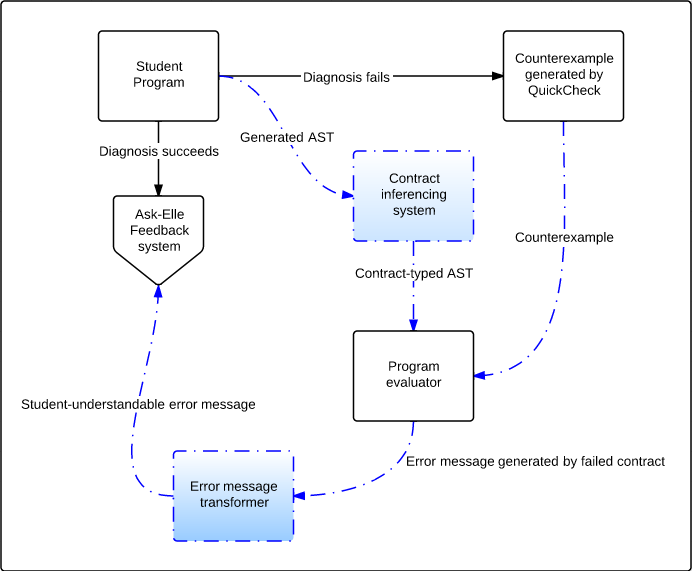
\includegraphics[width=0.5\textwidth]{Embed-Overview.png}
  \caption{Overview of steps involved in the contract inferencing system.}
\label{fig:EmbedOverview}
\end{figure}

Figure \ref{fig:EmbedOverview} depicts an overview of the steps involved in using the contract inferencing system.
The blue dashed-dotted arrows and boxes represent functionality that is not yet present in Ask-Elle, but is required for the contract inferencing system to be of use.
Let us step through the system and inspect the goals and requirements of each element in more detail.

Currently, if conventional 'diagnosis' of the student program fails, a QuickCheck example is generated, after which it is displayed to the user (this arrow is not shown).
Alongside the counterexample, the AST of the student program must be generated such that it can be used by the contract inferencing system.
The ASTs used by the Ask-Elle programming tutor and the contract inferencing system differ; Ask-Elle uses Helium as its back-end for Haskell, and Algorithm CW is based upon a small lambda language. So the first step towards embedding the system will be:

\begin{description}
	\item{\textbf{Step 1}} Modify and extend Algorithm CW to accept the AST generated by Ask-Elle, and embed it in Ask-Elle.
\end{description}

Initial work of this step has already been undertaken by research assistants (\todo{Who?}).
After completing Step 1, it should be possible to infer a contract for any arbitrary AST generated by Ask-Elle.

The next step is to use the contract-typed AST to generate an error message.
There are two ways of doing this:

\begin{enumerate}
	\item Use the QuickCheck-provided counterexample to transform the contract-typed AST directly, and then convert it back to an executable program and run it. We suspect that this functionality will be required for dependent function contracts.
	\item Convert the contract-typed AST back to an executable program immediately, and apply the counterexample to it.
\end{enumerate}

Replacing parts of the contract-typed AST with a counterexample was touched upon in Stutterheim's thesis, but an automated way of determining what should be replaced and where does not seem to be available.
Hence, this  is the next step:
\begin{description}
	\item{\textbf{Step 2}} Investigate an automated way of modifying the contract-typed AST with a counterexample, and implement this functionality.
\end{description}

After (not) modifying the contract-typed AST, it must be converted back into an executable program.
We assume the Helium-compiler has a way of feeding it an AST and returning an executable program.
However, keeping the well-known saying about assumptions in mind, we will have to investigate further:

\begin{description}
	\item{\textbf{Step 3}} Investigate if it is possible to feed a contract-typed AST to the Helium compiler. If not, investigate if this functionality can be implemented.
\end{description}

If all has gone well, we should end up with an error message generated by the Helium compiler, caused by a contract violation.
However, returning this error message to the student will not result in useful feedback.
Therefore, we must transform the error message by replacing the details of the contract violation with those of the function wrapped by the violated contract.
This transformed error message will be returned to the student. The final step of this subsection, then, is as follows:

\begin{description}
	\item{\textbf{Step 4}} Implement an error message transformer that "cleans up" the generated error message so it is understandable by the student, and feed it to the Ask-Elle feedback mechanism.
\end{description}

\subsection{Goal Two: Perform testing with students}

In August, Utrecht University hosts an Applied Functional Programming summer school.
This summer school course specifically targets students and participants who are not yet very knowledgeable about functional programming in general, and Haskell in particular.
This is an excellent opportunity to test the functionality described in Goal One.
Let us again go through each step that must be taken to complete this goal.

The first step is relatively simple, but nonetheless crucial:

\begin{description}
	\item{\textbf{Step 1}} Organize the practical aspects of the testing on time. Contact the coordinators of the summer school and request a time slot during which testing can take place.
\end{description}

After that, we must provide two versions of the Ask-Elle tutor: one with the new contract inferencing system embedded, and the original, unmodified one.
We require two versions to perform a simple A/B test: for each exercise, a version of Ask-Elle is randomly selected and presented to the student.
Thus, we require a way to randomly serve one of the versions to a student:

\begin{description}
	\item{\textbf{Step 2}} Prepare two versions of the Ask-Elle tutor, and set up access in such a way that, for each exercise, one of the versions is randomly served to the student.
\end{description}

After completing an exercise in Ask-Elle (there are around fifteen exercises in total), the student will fill out a very small survey if he or she encountered feedback containing a counterexample.
The feedback will be shown above the survey.
The following questions will then be visible below the feedback:

\fbox {
    \parbox{\linewidth}{
For each question, please mark the circle that corresponds with your opinion.
\begin{enumerate}
	\item The feedback above provided me with sufficient information to help me find the mistake in my code. \newline
[Strongly disagree] 0 - 0 - 0 - 0 - 0 [Strongly agree]
	\item The feedback above should indicate a more specific part of the code.\newline
[Strongly disagree] 0 - 0 - 0 - 0 - 0 [Strongly agree]
\end{enumerate}
    }
}

As this survey is quite small, it could be made multi-lingual if this makes students more inclined to take part in the survey.

With the results of these surveys, we are able to discern which version of Ask-Elle students prefer when they encounter feedback containing a counterexample.

So, our final steps for this goal are:

\begin{description}
	\item{\textbf{Step 3}} Build a small survey system that acquires any feedback containing a counterexample from the Ask-Elle tutor and presents the survey mentioned above, then writes the answers back to a database.
	\item{\textbf{Step 4}} Test the entire system beforehand, and ensure it is operational for use by the students.
	\item{\textbf{Step 5}} Collect survey results.
\end{description}

\subsection{Goal Three: Analyze the testing results and report findings}

Having collected the survey results, all that remains to be done is to analyze them and determine if the embedding of the contract inferencing system in Ask-Elle has increased the usefulness of feedback containing a counterexample provided to students, or not:

\begin{description}
	\item{\textbf{Step 1}} Analyze the survey results to answer the research question.
\end{description}

After processing the results, we will present our findings in a presentation, as is customary:

\begin{description}
	\item{\textbf{Step 2}} Report findings and problems encountered / lessons learned during this thesis in a presentation.
\end{description}

\section{Stretch Goals}
In case the goals described in section~\ref{sec:research-goals} require less time than was planned, there are a few stretch goals available:

\subsection{Goal One Stretch Goals}
\begin{itemize}
	\item Ask-Elle's normal analysis may fail because of a multitude of reasons.
Eta-expansion, commutativity, associativity and many other transformations that do not change the meaning of the program are currently unsupported by Ask-Elle.
Collecting and categorizing these problematic transformations would be great source of examples for future work in supporting these transformations.
	\item At the moment, there are only counterexamples available for Haskell, generated by QuickCheck. However, Ask-Elle focuses on functional languages in general. Generalizing the counterexample and contract inferencing interfaces may not be too big of a hassle and prove to be an ideal foundation for further future work.
	\item Building further upon the previous stretch goal, a toy implementation of another functional language in the tutor is a final ambitious stretch goal that could help lay bare any existing issues with Ask-Elle's architecture. There are multiple functional candidates available, such as Scheme, Erlang and Clojure, all of which are quite different from Haskell. As an added bonus, there exist QuickCheck ports for all of these languages.
\end{itemize}

\subsection{Goal Two Stretch Goals}

\begin{itemize}
	\item It may be of interest to extend the survey presented to students (or present a larger survey at the end of the exercise set) to learn more about how the students perceived Ask-Elle's performance.
However, this could increase the time needed for testing, and it remains to be seen if this extra time can be made available, if at all.
A starting point for a larger survey could be the original survey in Alex Gerdes' thesis \cite{Gerdes:2012:phd}.
	\item In case testing during the summer school course provides insufficient data (or data was unable to be collected for whatever reason), it may be desirable to perform additional testing. As Ask-Elle is designed to work from a web browser, testing and survey taking can be done remotely; identifying and contacting students interested in functional programming (inside and outside the university) may prove to be a valuable source of potential survey takers.
\end{itemize}

\section{Related Work}

Stutterheim's  \cite{Stutterheim:2013:thesis} thesis uses a dynamic contract library developed by Hinze et al. \cite{Hinze06typedcontracts}, whose work was inspired by Findler and Felleisen \cite{Findler:2002:CHF:583852.581484,Findler02behavioralsoftware}.
Degen et al. \cite{DegenThiemannWehr2009} demonstrate how all forms of dynamic contract monitoring (eager, semi-eager and lazy) are inherently flawed, either changing program behaviour or ignoring contract violations. The dynamic contract library of Hinze et al. is semi-eager. The article also touches upon Xu's \cite{Xu:2009:SCC:1594834.1480889} work on static contract systems for Haskell, and the authors argue that Xu's system is similar to the eager monitoring style they discuss in the article. Eager contract monitoring is preferred by the authors as all contracts defined in it are faithful: they will always evaluate to their actual value, which implies that, if a program terminates, all of the contracts within it will have evaluated to true.
 
Cousot et al. \cite{cousotabstract} have implemented automatic contract inference for method extraction, a common refactoring technique.
The inferred contract satisfies four requirements: (i) it is valid for the extracted method; (ii) the contract takes into account language and programmer assertions; (iii) the contract of the refactored code is as precise as the non-refactored code, and (iv) the contract is as general as possible.
The authors use an iterative approximation algorithm to attain contracts that fulfil these requirements, and prove that an exact solution is uncomputable.

Rondon et al. \cite{rondon2008liquid} have developed a set of data types called Logically Qualified Data Types, often shortened to Liquid Types.
These are an example of Refinement Types.
Using liquid types, they are able to embed a decidable subset of dependent typing functionality in a Hindley-Milner typing system.
With only the HM types and a predefined set of logical qualifiers, their algorithm is able to infer liquid types, which are dependent types that consist of conjunctions of the aforementioned logical qualifiers.
After inferring these liquid types, they can be resolved using an SMT solver.
In the end, one ends up with the strongest constraint possible on the expression that can be generated with the provided set of logical qualifiers.
Implementations of liquid typing are available for OCaml \cite{rondon2008liquid} and Haskell (using GHC) \cite{rondon2013refinement}.
The Haskell implementation is able to provide feedback if type checking fails, indicating the position(s) in the source code where things have gone wrong.
Additionally, a HTML file is generated of the processed source code annotated with the inferred types.

Terauchi \cite{terauchi2010dependent} also builds upon the recent developments in refinement types to present a system that is able to infer dependent types for a subset of the OCaml language without external input.
Instead of taking a user-provided set of formulas, the algorithm uses counterexample guided abstraction refinement (CEGAR) to iteratively refine a lattice of candidate dependent types.
Counterexamples are parts of the program that are untypable with the current lattice of candidate types.
The algorithm then attempts to type the program with all available types instead of the lattice.
If typing succeeds, the new candidates are added to the lattice and a new counterexample is selected.
If it fails, then the program is untypable.
As the algorithm itself generates the set of candidates, users can be sure that if the program is untypable, it really is untypable.
On the other hand, because the types are inferred automatically, they are not necessarily the strongest types available.

Ranjit et al. \cite{jhala2010refinement} take another route to attain refinement types: they first attain refinement type constraints using the implementation of Rondon et al. \cite{rondon2008liquid}, and then translate these types to a first-order imperative program.
Iff the assertions of this imperative program hold, the higher-order program typechecks.
This verification can be done using several abstract interpretation techniques (of which CEGAR is one), which have readily available implementations for imperative languages.
The proof of safety of the imperative program translates to the solutions of the refinement type constraints.
Thus, these can be used to annotate the original higher-order program, obtaining the refinement types.

The articles of Dimoulas \& Felleisen \cite{Dimoulas:2011:CSH:2039346.2039348} and Greenberg et al. \cite{Greenberg:2010:CMM:1707801.1706341} provide an excellent overview of recent developments pertaining to contracts, as well as as detailed comparisons between the different libraries and frameworks. \cite{Dimoulas:2011:CSH:2039346.2039348} also goes into greater detail of the semantics of contract satisfaction.


\section{Acknowledgements}
I would like to thank Johan Jeuring and Wouter Swierstra for their master thesis suggestions and for helping me delineate the initial research goals of this thesis proposal. Johan also suggested several very interesting papers to me for use in the related work section.

\bibliographystyle{unsrtnat}
\bibliography{doc}

\end{document}